% Development

% Main chapter title
%\chapter[toc version]{doc version}
\chapter{Development}

% Short version of the title for the header
%\chaptermark{version for header}

% Chapter Label
% For referencing this chapter elsewhere, use \ref{ChapterTemplate}
\label{Development}

This chapter describes the development of the timetable system, formulating the problem, discussing the implementation of the \ac{mcts} and \ac{hc} hybrid approach, detailing the design choices, algorithmic improvements and integration efforts made throughout the project.

\section{Problem Formulation}

The entities in the problem are listed below:

\begin{itemize}
	\item \textbf{Periods, \(P = \{P_0, P_1, ..., P_|_P_|_-_1\}\):} Days are divided into fixed timeslots, with periods consisting of a day and a timeslot.

		%\unsure[inline]{In the previous work, there is no periods. There are weekdays, a start time and an end time. For now, in the current approach, an event is only associated with a period of one hour and without any link to previous work. If I implement this concept to previous work, an event should be assigned to one or more half-hour periods.}

	\item \textbf{Rooms, \(R = \{R_0, R_1, ..., R_|_R_|_-_1\}\):} Each room has a capacity and a type.
		\begin{itemize}
			%\item Occupation (the room may be utilized for non-teaching reasons, such as exams) (TODO)
			\item Capacity (number of seats)
			%\item Type (TODO)
		\end{itemize}

	\item \textbf{Lecturers, \(L = \{L_0, L_1, ..., L_|_L_|_-_1\}\):} 
		\begin{itemize}
			%\item Office
			\item Availability
			%\item Restriction (availability and TODO: preferences for periods)
		\end{itemize}

	\item \textbf{Events, \(E = \{E_0, E_1, ..., E_|_E_|_-_1\}\):} Represent the events to be scheduled (usually a lecture). Each event has associated attributes:
%		\begin{multicols}{2}
%		\textbf{Previous work:}
%		\begin{itemize}
%			\item Start and end time
%			\item Weekday
%			\item Duration
%			\item Lecturer
%			\item Room
%		\end{itemize}
%		\columnbreak
%		\textbf{TODO: adicionar ao trabalho anterior?}
		\begin{itemize}
        		\item Capacity (number of students)
        		\item Number of lectures
        		\item Minimum working days (days over which the events of the same course should be spread)
        		\item Available periods
        		\item Priority
        		\item Lecturer
        		\item Period (day, timeslot)
 			\item Room
		\end{itemize}
%		\end{multicols} 

	\item \textbf{Blocks, \(B = \{B_0, B_1, ..., B_|_B_|_-_1\}\):} A block may represent a group of related events. Usually represents all events from the same curriculum, which is a set of courses in a study program.
\end{itemize}

\subsection{Constraints}

There are several hard and soft constraints that affect the creation of \ac{fcup} timetables. The following hard and soft constraints were selected, drawing inspiration from those of \ac{itc-2007}:

\textbf{Hard constraints:}

\begin{itemize}
	\item \textbf{H1:} Events belonging to the same course must be scheduled and must be assigned to distinct periods.
	\item \textbf{H2:} Two events can be scheduled in the same room, but only if they are in different periods.
	\item \textbf{H3:} Events of the same curricula, or taught by the same lecturer, must be scheduled in different periods.
	\item \textbf{H4:} If a lecturer is unavailable in a given period, then no events can be taught by this lecturer in that period.
%	\item \textbf{TODO H5:} If a room is unavailable in a given period, then no events can be scheduled in that period.
%	\item \textbf{TODO H6:} Lecturers and students must have a free lunch period.
\end{itemize}

\textbf{Soft constraints:}

\begin{itemize}
	\item \textbf{S1:} Events of the same course should be spread into the given minimum number of days.
	\item \textbf{S2:} Events belonging to the same curriculum should be in consecutive periods.
	\item \textbf{S3:} The capacity of the room should be higher or equal than the capacity of the event.
	\item \textbf{S4:} All events of a course should be given in the same room.
\end{itemize}

The problem is defined as a maximization problem, with the algorithm attempting to minimize soft constraint violations while strictly adhering to hard constraints.

\section{Monte Carlo Tree Search}

%This section describes the key algorithmic components of the system, particularly the hybrid \ac{mcts} with \ac{hc} approach.

%(...)

\subsection{Search Space}

The search space, \(S\),  for this problem is large as it involves a product of all possible event-period-room combinations: \[S = E \cdot P  \cdot R,\] where \(E\) is the set of events, \(P\) is the set of periods (day, timeslot), and \(R\) is the set of rooms.

To reduce the search space, unavailable periods and unavailable rooms for a chosen period are discarded immediately in the \ac{mcts} \(expansion\) phase.

\subsection{\ac{mcts} Tree}

\begin{figure}
      \centering
      \includegraphics[width=0.7\columnwidth]{Development/MCTS_tree.jpg}
      \caption[MCTS tree]
      {MCTS tree}
      \label{fig:mcts_tree}
\end{figure}

Figure \ref{fig:mcts_tree} illustrates the basic structure of the \ac{mcts} tree. The root represents the initial state, where no events have been assigned. The first level corresponds to assigning the first event, \(E_0\), to various \(P\) and \(R\). Each child node represents a specific assignment (\((E_0,P_0,R_0),...,(E_0,P_|_P_|_-_1,R_|_R_|_-_1)\)). Subsequent levels correspond to the sequential assignment of events \(E_1, E_2, ..., E_|_E_|_-_1\).

\subsubsection{Tree Nodes}

A node is composed of the following attributes:

\begin{itemize}
\item A \textbf{path} is a dictionary that represents the sequence of actions leading to a node. The root is the only node that has an empty path.

\item A \textbf{parent} is a reference to the parent node, allowing the tree structure to be navigated upwards. The root is the only node that does not have a parent.

\item \textbf{Children} is initialized as an empty list at first but will later hold references to the node's child nodes. 

\item The \textbf{expansion limit} specifies the maximum number of children that a node can have, which helps control the expansion process. It is estimated based on the number of available rooms per period for the next event. A value of zero indicates that the node cannot be expanded further.

\item \textbf{Visits} is initialized to 0, tracking the number of times a node has been visited.

\item The \textbf{hard and soft scores} are both initialized to 0, representing the cumulative hard and soft scores for a node, which are used to evaluate the quality of the node's state.

\item The \textbf{best hard and soft penalty results} are initialized to negative infinity, representing the best hard and soft penalty results encountered for a node. These attributes will be updated during the algorithm as better results are found. 
\end{itemize}

\subsection{Events Allocation}

Events are sorted in advance so that the most difficult event to place is placed first in the tree. The priority of an event (Formula \ref{priority}) is calculated based on:

\begin{itemize}
\item The difference between the number of lectures and minimum working days to prioritize events with more lectures spread over fewer days;
\item The number of available periods, as having more available periods indicates fewer scheduling restrictions;
\item The capacity of an event, which implies that events with greater capacity have higher priority;
\item The number of curricula in which the event is, as events that appear in more curricula are more difficult to allocate.
\end{itemize}

If two or more events have the same priority score, they are ordered randomly.

\begin{equation}
  \begin{aligned}
	Priority = (\#lectures - \#min\_working\_days) \cdot 4 \\
	           - \#available\_periods \cdot 3 \\
	          + capacity \cdot 2 \\
	          + \#blocks\label{priority}
  \end{aligned}
\end{equation}

%I have tried other priority formulas...

\subsection{Periods and Rooms Allocation}

Initially, our approach to allocating periods and rooms in the \ac{mcts} tree followed a structured sequence. This method aimed to explore all possible (period, room) combinations based on the number of children of the current node being expanded. However, as we progressed, this approach started to fail when the availability of rooms varied across different periods. A refined approach was then developed to address these limitations more robustly.

\subsubsection{Initial Periods and Rooms Allocation Approach}

In the initial approach, each event assignment generated in the \ac{mcts} tree follows a structured sequence for period and room allocation. 
Let:
\begin{itemize}
\item \(n\) be the number of children of the current node being expanded;
\item \(AP\) the number of available periods;
\item \(AR\) the number of available rooms. 
\end{itemize}

The assignment is determined as follows:

\begin{itemize}
	\item The period index was selected using: 
		\begin{equation}
		n \mod AP\label{period_allocation}
		\end{equation}
	
	\item The room index was selected using:
		\begin{equation}
		\frac{n}{AP} \mod AR\label{room_allocation}
		\end{equation}
\end{itemize}

This resulted in a deterministic exploration order. For instance, if \(AP = 3\) and \(AR = 2\), the assignment would be:
\[
\begin{aligned}
n = 0 &\Rightarrow P_0, R_0 \\
n = 1 &\Rightarrow P_1, R_0 \\
n = 2 &\Rightarrow P_2, R_0 \\
n = 3 &\Rightarrow P_0, R_1 \\
n = 4 &\Rightarrow P_1, R_1 \\
n = 5 &\Rightarrow P_2, R_1 \\
\end{aligned}
\]

This approach assumes that the number of children will always perfectly expand all (period, room) combinations, but it fails when the search space is reduced, resulting in different periods having different available rooms.

Consider the following scenario:
\begin{itemize}
\item Available Periods = \([(0,1), (3,2)]\)
\item Rooms at (0,1) = \(['C', 'D', 'E', 'F', 'G']\) (5 rooms)
\item Rooms at (3,2) = \(['B']\) (1 room)
\end{itemize}

Here, \(AP = 2\), but the number of available rooms (\(AR\)) depends on the period. The expansion limit is 6, thus we compute assignments from \(n = 0\) to \(n = 5\):

\[
\begin{aligned}
n = 0: &\quad P_0 = (0,1),\quad R_0 = 'C' \quad &\text{(Valid)} \\
n = 1: &\quad P_1 = (3,2),\quad R_0 = 'B' \quad &\text{(Valid)} \\
n = 2: &\quad P_0 = (0,1),\quad R_1 = 'D' \quad &\text{(Valid)} \\
n = 3: &\quad P_1 = (3,2),\quad R_0 = 'B' \quad &\text{(Invalid: Duplicate)} \\
n = 4: &\quad P_0 = (0,1),\quad R_2 = 'E' \quad &\text{(Valid)} \\
n = 5: &\quad P_1 = (3,2),\quad R_1 = 'B' \quad &\text{(Invalid: Duplicate)} \\
\end{aligned}
\]

Because room availability is period-specific, the formula produces duplicate assignments when \(AR\) is not consistent across all periods.

\subsubsection{Final Periods and Rooms Allocation Approach}

To overcome these limitations, instead of computing the (period, room) combinations via index math, we pre-compute all valid combinations once. This method produces a flat list of unique, valid assignments, and expansion always proceeds without duplication.

Moreover, periods that are less frequently available across all events are given higher priority. In this way, the algorithm reduces the risk of future conflicts, guiding the tree toward more constrained decisions early. For each period, available rooms are also sorted by how closely their capacity matches the event’s requirements, minimizing wasted space and increasing flexibility in room usage.

\subsection{Methodology}

The \ac{mcts} algorithm consists of four phases: \(selection\), \(expansion\), \(simulation\), and \(backpropagation\). Each phase plays a critical role in exploring the search space and updating the tree structure with the simulation outcomes. Figure \ref{fig:mcts_steps} provides a high-level overview of these four phases in the \ac{mcts} process.

\begin{figure}[H]
      \centering
      \includegraphics[width=1.1\columnwidth]{Development/MCTS_Steps.jpg}
      \caption[MCTS steps]
      {MCTS steps}
      \label{fig:mcts_steps}
\end{figure}

\subsubsection{Selection}

The \(selection\) phase (Algorithm \ref{selection}) begins at the root and traverses the tree by iteratively selecting the best child nodes until a terminal (leaf) node is reached. A node is considered terminal if either it cannot be expanded further (i.e., its expansion limit is zero) or if it has reached the maximum depth (i.e., all the events have been assigned). Conversely, a node is deemed fully expanded if either its expansion limit is zero or if the number of its children equals its expansion limit. When the traversal encounters a node that is not fully expanded, the process stops, and that node is selected for further expansion.

The best child node (Algorithm \ref{best_child}) is determined by applying the \ac{uct} formula (\ref{uct_formula}). However, as the problem has two goals, maximizing the hard constraints first and then the soft constraints, the \ac{uct} formula was applied differently. Initially, the algorithm computes the weights for each child node using the hard score. Among the children with the highest hard score, the weights are recalculated based on the soft score. The child node with the highest weight in this second calculation is selected as the best child. However, if all of a node's children have reached their expansion limit, the algorithm backtracks: if the current node has a parent, the current node expansion limit is set to zero, and it moves up to the parent. Reaching the root indicates that the entire tree is fully expanded.

\begin{algorithm}
\caption{Selection}\label{selection}
\begin{algorithmic}[1]
\Procedure{SELECTION}{}
    \State current\_node $\gets$ root
    \While{not current\_node.\textit{is\_terminal\_node}(\textit{len}(events))}
        \If{not current\_node.\textit{is\_fully\_expanded}()}
            \State \textbf{break}
        \EndIf
        \State unflagged\_children $\gets$ [child \textbf{for each} child \textbf{in} current\_node.children \textbf{if} child \textbf{and} child.expansion\_limit $\neq$ 0]
        \If{unflagged\_children is empty}
            \If{current\_node.parent exists}
                \State current\_node.expansion\_limit $\gets 0$
                \State current\_node $\gets$ current\_node.parent
            \Else
                \State \Return False
            \EndIf
        \Else
            \State current\_node $\gets$ current\_node.\textit{best\_child}(unflagged\_children)
        \EndIf
    \EndWhile
    \State self.current\_node $\gets$ current\_node
    \State \Return True
\EndProcedure
\end{algorithmic}
\end{algorithm}

\begin{algorithm}
\caption{Best Child}\label{best_child}
\begin{algorithmic}[1]
\Function{BEST\_CHILD}{unflagged\_children, c\_param = 1.4}
    \State choices\_weights $\gets$ [$\frac{child.score\_hard}{child.visits} $+$ c\_param $\cdot \sqrt{\frac{2\ln(self.visits)}{child.visits}}$ \textbf{for each} child \textbf{in} unflagged\_children]
    \\
    \State max\_weight $\gets$ \textit{max}(choices\_weights)
    \State best\_children $\gets$ [unflagged\_children[i] \textbf{for each} i, weight \textbf{in} \textit{enumerate}(choices\_weights) \textbf{if} weight = max\_weight]
    \\
    \State choices\_weights $\gets$ [$\frac{child.score\_soft}{child.visits} $+$ c\_param $\cdot \sqrt{\frac{2\ln(self.visits)}{child.visits}}$ \textbf{for each} child \textbf{in} best\_children]
    \\
    \State \Return best\_children[\textit{index\_of}(\textit{max}(choices\_weights))]
\EndFunction
\end{algorithmic}
\end{algorithm}

\subsubsection{Expansion}

The \(expansion\) phase (Algorithm \ref{expansion}) is responsible for expanding the node previously selected by assigning the next event to a valid (period, room) combination and creating a corresponding child node.

The next event to schedule is determined by the depth of the current node. For the selected event, the algorithm gathers the available (weekday, timeslot) combinations and filters suitable rooms for each period (Algorithm \ref{find_available_rooms}), based on the event’s capacity requirements and current room occupation.

A list of valid (period, room) combinations is generated. If no such combinations exist or the node has already been expanded for all possibilities, expansion is terminated, and the node is marked as fully expanded.  

A combination is selected based on the number of already-expanded children. A new path is constructed by assigning the selected period and room to the event.

Before proceeding, the algorithm evaluates the partial timetable (i.e., the new path) against a global hard penalty threshold. If the new assignment violates hard constraints resulting in a penalty below the threshold, a null child is added to indicate that the expansion stopped for that branch. This pruning condition reduces unnecessary exploration.

If the expansion continues, the algorithm estimates the number of valid (period, room) combinations for the next event. This value is stored as the child’s expansion\_limit to guide future branching.

Finally, a new child node is created with the updated path and expansion limit. This new node is added to the tree, and the current node is updated to this newly created node.

\begin{algorithm}
\caption{Expansion}\label{expansion}
\begin{algorithmic}[1]
\Function{EXPANSION}{}
    \State event $\gets$ events[current\_node.\textit{depth}()]
    \State available\_periods $\gets$ event["Available\_Periods"]
    \\
    \If{available\_periods is empty}
        \State current\_node.expansion\_limit $\gets$ 0
        \State \Return False
    \EndIf
    \\
    \State rooms\_by\_period $\gets$ \textit{find\_available\_rooms}()
    \State period\_room\_combinations $\gets$ [(weekday, timeslot, room) \textbf{for} (weekday, timeslot), rooms in room\_by\_period.\textit{items()}]
    \\
    \If{period\_room\_combinations is empty \textbf{or} current\_node is fully expanded}
        \State current\_node.expansion\_limit $\gets$ 0
        \State \Return False
    \EndIf
    \\
    \State new\_weekday, new\_timeslot, new\_room $\gets$ period\_room\_combinations[len(current\_node.children)]
    \State new\_path $\gets$ \textit{copy}(current\_node.path)
    \State new\_path[event["Id"]] $\gets$ \{**event, "RoomId": new\_room, "WeekDay": new\_weekday, "Timeslot": new\_timeslot\}
    \\
    \State new\_expansion\_limit $\gets$  = \textit{calculate\_expansion\_limit}(new\_path)
    \State \textbf{if} new\_expansion\_limit is None: \Return False
    \\
    \State child\_node $\gets$ MCTSNode(expansion\_limit = expansion\_limit, parent = current\_node, path = new\_path)
    \State current\_node.children.\textit{append}(child\_node)
    \State current\_node $\gets$ child\_node
    \State \Return True
\EndFunction
\end{algorithmic}
\end{algorithm}

\begin{algorithm}
\caption{Find Available Rooms}\label{find_available_rooms}
\begin{algorithmic}[1]
\Function{FIND\_AVAILABLE\_ROOMS}{event\_capacity, rooms, events, available\_periods}
    \State period\_room\_availability $\gets$ \{period: \textit{set}(rooms.keys()) \textbf{for each} period \textbf{in} available\_periods\}
    \For{\textbf{each} other\_event \textbf{in} events}
        \State occupied\_period $\gets$ (other\_event["WeekDay"], other\_event["Timeslot"])
        \If{occupied\_period \textbf{in} period\_room\_availability}
            \State period\_room\_availability[occupied\_period].\textit{discard}(other\_event["RoomId"])
        \EndIf
    \EndFor
    \\
    \State suitable\_rooms $\gets$ \{room\_id \textbf{for each} room\_id, room \textbf{in} rooms.items() \textbf{if} room["Capacity"] $\geq$ event\_capacity\}
    \\
    \For{\textbf{each} period \textbf{in} available\_periods}
        \If{period\_room\_availability[period] is not empty}
            \State intersected $\gets$ period\_room\_availability[period] $\cap$ suitable\_rooms
            \If{intersected is not empty}
                \State sorted\_rooms $\gets$ \textit{sort}(intersected, by (room["Capacity"] - event\_capacity))
            \Else
                \State sorted\_rooms $\gets$ \textit{sort}(period\_room\_availability[period], by $|$room["Capacity"] - event\_capacity$|$)
            \EndIf
            \State period\_room\_availability[period] $\gets$ sorted\_rooms
        \EndIf
    \EndFor
    \\
    \State \Return period\_room\_availability
\EndFunction
\end{algorithmic}
\end{algorithm}

\subsubsection{Simulation}

The \(simulation\) phase estimates the value of multiple actions, in this case, distinct event allocations, which will guide the selection and expansion steps in future iterations. 

A random event allocation approach was initially explored but produced suboptimal results. Therefore, a more structured method was implemented.

The \(simulation\) function (Appendix \ref{AppendixA} Algorithm \ref{simulation}) starts by creating a copy of the current node's path, which contains the events already scheduled. It then identifies the remaining events, i.e., events that have not been assigned yet. These remaining events are sorted based on two criteria:
\begin{enumerate}
\item Whether they were previously unassigned in prior simulations, to prioritize harder-to-schedule events.
\item Their priority, ensuring that more critical events are allocated first.
\end{enumerate}

For each unvisited event, the best available period and room combination is sought. The approach iterates through all the available periods and rooms, calculating the hard and soft penalties for each combination. During the calculation of the soft penalty, the importance of compactness (i.e., minimizing the time between related events) is adjusted, with a higher weight applied as the algorithm progresses.The combination with no hard penalties and the lowest soft penalty is selected as the best option. If multiple optimal choices exist, one is randomly selected. The event is then updated with the selected room, weekday, and timeslot. If no valid allocation is found, the event will have higher priority in the next simulation.

After scheduling all events, the simulation result is calculated, and the best and worst penalty scores are then updated based on these results. If a new best result is found, the timetable is saved to a file. If a new best result is found and the hard penalty is zero, indicating a feasible solution, the \ac{hc} algorithm (section \ref{hill_climbing_section}) is used to further optimize the timetable.

\subsubsection{Backpropagation}

The \(backpropagation\) phase (Algorithm \ref{backpropagation}) updates the tree based on the simulation results. 

It starts from the current node, which is the leaf node where the simulation occurred, and moves up until reaching the root node. During this process, it performs updates for each node in the path, including incrementing the number of visits and updating the hard and soft scores with the simulation results. 

\begin{algorithm}
\caption{Backpropagation}\label{backpropagation}
\begin{algorithmic}[1]
\Function{BACKPROPAGATION}{simulation\_result\_hard, simulation\_result\_soft}
    \State node $\gets$ current\_node
    \While{node $\neq$ None}
        \State node.visits $+=$ 1
        \State node.score\_hard $+=$ simulation\_result\_hard
        \State node.score\_soft $+=$ simulation\_result\_soft
        \State node $\gets$ node.parent
    \EndWhile
\EndFunction
\end{algorithmic}
\end{algorithm}

\subsection{Normalization}

The normalization formula \ref{normalization_formula} is applied to both hard and soft constraints to standardize the simulation results \cite{pedroso_tree_2015}:

\begin{equation}
N(n) = \frac{e^a - 1}{e - 1}, \quad \text{with } a = \frac{best\_penalty_n - worst\_penalty}{best\_penalty - worst\_penalty},\label{normalization_formula}
\end{equation}
where \(best\_penalty\) and \(worst\_penalty\) represent the best and the worst simulation results in the entire tree, and \(best\_penalty_n\) is the best simulation result under node \(n\).

This formulation ensures that the best simulation result is mapped to a value close to one, while the worst is mapped to zero.

\section{Hill climbing}\label{hill_climbing_section}

The \ac{hc} algorithm (Appendix \ref{AppendixA} Algorithm \ref{run_hill_climbing}) is applied as a local search method to further optimize the timetable obtained from the \ac{mcts} simulation phase. This approach refines an initially feasible solution by iteratively exploring small modifications to enhance overall quality.

To maintain the structure established during the tree search, \ac{hc} only modifies events that were not allocated in the \ac{mcts} phase. This ensures that the global search strategy remains intact while improving suboptimally placed events by the simulation phase.

\subsection{Neighborhoods}

After finding a feasible solution with \ac{mcts}, \ac{hc} refines the solution by exploring neighboring states. The algorithm explores the solution space using six different types of neighbors inspired by the \ac{itc-2007} track 3 winner \cite{muller_itc2007}:

\begin{itemize}
\item \textbf{Period move:} Change the timeslot and weekday of an event while keeping the same room.
\item \textbf{Room move:} Change the room of an event while keeping the same timeslot and weekday.
\item \textbf{Event move:} Change both the room and timeslot of an event.
\item \textbf{Room stability move:} Assign all events of the same course to the same room if possible.
\item \textbf{Compactness move:} Move an event to a timeslot adjacent to another event of the same curriculum.
\item \textbf{Minimum working days move:} Spread a course's events across more days to avoid teaching all lectures in a short period.
\end{itemize}

Each move has a weight, which affects how often it is chosen. Period, room and event moves appear to be the most effective, consequently they have a higher weight than the others.

\subsection{Methodology}

The \ac{hc} approach follows the following steps:

\begin{enumerate}
\item Starts with an initial complete timetable with no hard constraints violated.
\item Repeatedly selects a random neighborhood move, based on the assigned weights.
\item Applies the move and evaluates the new timetable.
\item If the new timetable is better, it keeps the changes; otherwise, it reverts them.
\item Stops when:
	\begin{itemize}
	\item A timetable satisfying all hard and soft constraints is found.
	\item No improvements are identified after a predefined number of idle iterations (HC\_IDLE = 5000).
	\item The time limit is reached.
	\end{itemize}
\end{enumerate}

\section{Diving}

To improve effectiveness in timetable generation, we also implemented a diving strategy in \ac{mcts}.

Figure \ref{fig:diving} illustrates the \ac{mcts} process with the diving strategy over seven iterations. Initially, the algorithm begins with the root node and an empty queue. Every time the queue is empty, the \ac{uct} formula is applied. Since the queue is empty, the simulations queue is also empty. 

\begin{figure}
      \centering
      \includegraphics[width=\columnwidth]{Development/MCTS_Diving.jpg}
      \caption[Diving approach]
      {Diving approach}
      \label{fig:diving}
\end{figure}

\section{Front-end}

The development process involved several adaptations and refinements. Initially, the previous work was analyzed and made functional, serving as a baseline for the new system. 

The \ac{mcts} algorithm was being developed while also being integrated into the front-end  interface intended to showcase the project. However, as the focus shifted towards adapting it to the \ac{itc-2007} track 3 benchmark for performance evaluation and fine-tuning the algorithm, the front-end development gradually lost priority. As the algorithm evolved and diverged significantly from its original form, aligning it with the prior work proved difficult. Consequently, continuing its development would be time-consuming and ultimately not worthwhile, as it was primarily intended for demonstration purposes. Instead, the system should be directly integrated into the sigarra\footnote{https://sigarra.up.pt/up/pt/web_page.inicial} website.

%\begin{figure}
%    \centering
%      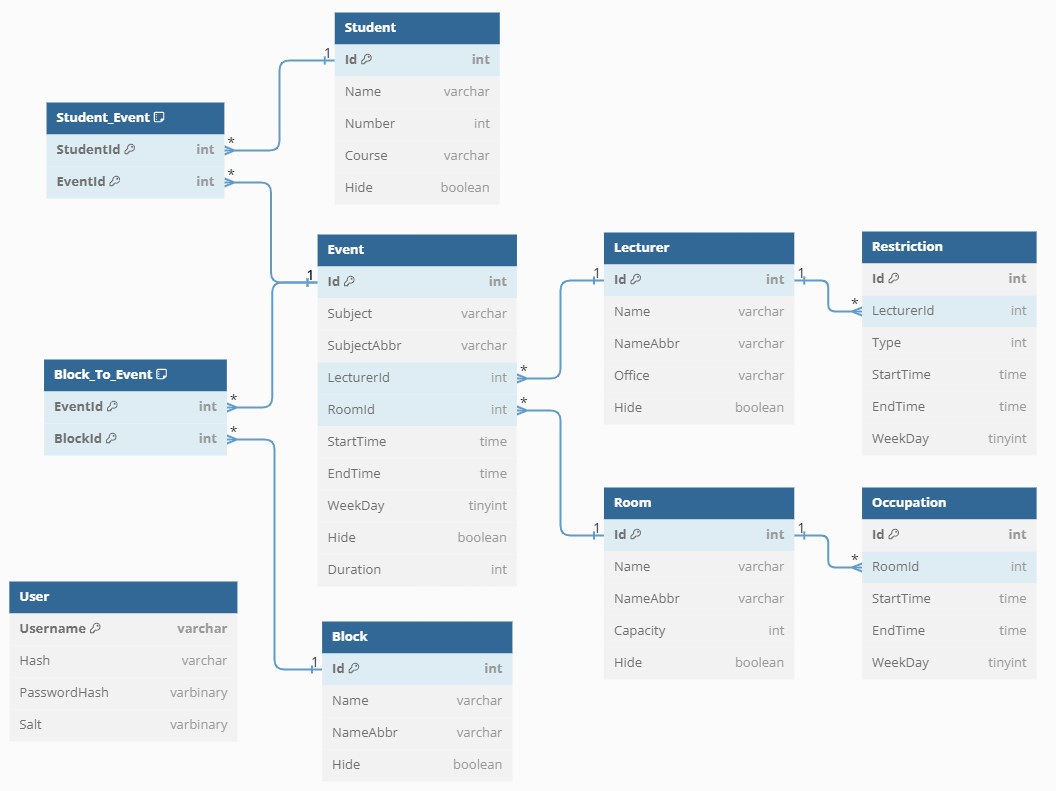
\includegraphics[width=1.1\columnwidth]{Development/uml.png}
%      \caption[UML]
%      {UML}
%      \label{fig:uml}
%\end{figure}